\documentclass[11pt]{article}
\usepackage[margin=1in]{geometry}

% Core packages
\usepackage{amsmath,amssymb}
\usepackage{booktabs}
\usepackage{graphicx}
\usepackage{tabularx}
\usepackage{xcolor}
\usepackage[hidelinks]{hyperref}
\usepackage{subcaption}
\usepackage[strings]{underscore}
\graphicspath{{figures/}}

% Paragraphs
\setlength{\parindent}{0pt}
\setlength{\parskip}{0.65\baselineskip}

\newcommand{\bigO}{\mathcal{O}}

\title{Bigger Bird: Evaluation of Content-Aware Sparse Attention}
\author{University of Toronto Machine Intelligence Student Team (UTMIST)}
\date{May--June 2026}

\begin{document}
\maketitle

\begin{abstract}
This report evaluates content-aware sparse-attention mechanisms for reducing the
quadratic cost of Transformer self-attention while preserving task quality. We
compare a dense BART baseline with routing, block-sparse, token-dropping,
layer-adaptive, and Bigger Bird variants on IMDb sentiment classification, using
an isolated attention-kernel benchmark (128--32{,}768 tokens, CUDA, 10 timing
trials) alongside end-to-end training and inference runs (256--65{,}536 tokens).
Layer-Adaptive Sparsity, DeepSeek Top-k routing, and Grouped-Query Sparse
attention are 2.2--4.6$\times$ faster than dense attention in isolated kernel
time by 4096 tokens and 17$\times$ faster at 16{,}384 tokens, where dense
attention itself runs out of memory by 32{,}768 tokens. At the task level,
Dynamic Context achieves the best IMDb F1 (0.942 at 1024 tokens, versus 0.894
for dense attention) with substantially lower inference latency (5.35~ms versus
13.18~ms), while Token Dropping gives the best long-context resource profile,
remaining within 0.048 F1 of dense attention at 32{,}768 tokens while using
82.5\% less peak memory and completing the only recorded 65{,}536-token IMDb
run. Long Range Arena (LRA) and RULER tracks are also reported briefly as
supplementary, exploratory evidence; the main quantitative conclusions of this
report are scoped to IMDb.
\end{abstract}

\newpage
\tableofcontents

\newpage
\section{Introduction}

Transformer models rely on self-attention to connect each token with every
other token in a sequence. Dense self-attention forms an $n\times n$ attention
matrix, giving it $\bigO(n^2)$ comparison and memory cost in sequence length
$n$. This is a practical bottleneck for long documents even when the
underlying model is otherwise small enough to train comfortably at short
lengths.

Bigger Bird investigates content-aware sparse attention as an alternative to
paying this quadratic cost everywhere. The guiding idea is to spend computation
on the connections that are likely to matter rather than applying one fixed
dense pattern uniformly. Sixteen numbered experiments (0--15) and a related
family of BigBird/Bigger Bird ablations were benchmarked, spanning low-rank
top-$k$ routing, block-sparse routing, dynamic global tokens, layer-adaptive
sparsity, token dropping, grouped-query attention, native sparse attention,
hierarchical shard attention, a BART-based unified Bigger Bird design with
learned-gate global selection, and a second Bigger Bird design built directly
on the BigBird-RoBERTa backbone that instead uses diversity-aware local
selection (MMR), submodular (facility-location) global selection, and biased
random teleports. This report first lays out the methodology -- the full set
of architectures evaluated and the protocol used to evaluate them -- and then
presents the resulting quantitative results.

\section{Objectives}

The evaluation pursues four objectives, each tied to a corresponding research
question addressed in Section~\ref{sec:methodology}:

\begin{enumerate}
  \item determine whether sparse methods retain the predictive quality of dense
  BART attention on IMDb sentiment classification;
  \item measure how attention-kernel time, inference latency, training time,
  and peak memory change as sequence length grows from shorter (128) to longer (65{,}536) tokens;
  \item identify quality--efficiency trade-offs and the sequence-length
  crossover points at which sparse attention overtakes dense attention; and
  \item isolate which routing and adaptation mechanisms are the strongest
  candidates for continued Bigger Bird development.
\end{enumerate}

\section{Chosen Dataset}
\label{sec:dataset}

\textbf{IMDb} binary sentiment classification is the primary evaluation
dataset used throughout this report. It provides an interpretable setting in
which F1 and accuracy can be compared across attention mechanisms at
controlled, fixed sequence lengths (256 through 65{,}536 tokens).

A number of additional \textbf{Long Range Arena (LRA)} (ListOps and byte-level
Text) and \textbf{RULER}-style needle-in-a-haystack retrieval runs were also
collected. These tracks are reported only briefly in this document as
exploratory, supplementary evidence: LRA quality is generally low and unstable
across sparse methods at this stage (e.g.\ ListOps F1 stays below 0.07 for
nearly every method at every length), and RULER results are dominated by a
single method (Dynamic Context, Section~\ref{exp:dynamic-context}), which
reaches perfect retrieval (F1~=~1.0, accuracy~=~1.0) at 4096 tokens across all
three tested needle depths (0.1, 0.5, 0.9) but degrades sharply at longer
context (F1~$\leq$~0.03 from 8192 tokens onward). Because LRA and RULER runs
differ from the IMDb runs in task definition, training schedule, and sample
count, they are not used to support the main quantitative conclusions of this
report, which are scoped to IMDb.

\section{Methodology}
\label{sec:methodology}

This section describes every attention architecture evaluated, followed by
the experimental protocol -- the sequence lengths, tasks, and measurement
conditions -- under which each architecture was run. Quantitative results for
each architecture are reported separately in Section~\ref{sec:results}.

\subsection{Model Architectures}
\label{sec:architectures}

Table~\ref{tab:taxonomy} groups the sixteen evaluated attention mechanisms by
family. Each is described architecturally below, with its default
hyperparameters and asymptotic complexity, and without reference to its
measured results.

\begin{table}[ht]
  \centering
  \caption{Taxonomy of evaluated attention mechanisms.}
  \label{tab:taxonomy}
  \begin{tabularx}{\textwidth}{@{}l>{\raggedright\arraybackslash}Xl@{}}
    \toprule
    Family & Representative mechanism & Experiments \\
    \midrule
    Reference & Dense BART self-attention & 0 \\
    Routed sparse & Low-rank top-$k$, block routing, grouped-query routing
      & 1, 4, 6, 10 \\
    Adaptive computation & Layer schedules, token dropping, dynamic context
      & 7, 8, 13, 14 \\
    Hybrid sparse & Windows, global tokens, speculation, NSA, S2-HHST
      & 2, 3, 9, 11, 12 \\
    Bigger Bird (BART backbone) & Local MMR + learned-gate globals + teleports
      & 5 \\
    Bigger Bird (BigBird-RoBERTa backbone) & Local MMR + facility-location
      globals + block-wise teleports & 15 \\
    \bottomrule
  \end{tabularx}
\end{table}

Experiments 11 and 12 are recorded as unfinished (``TODO'') in the current
codebase. Their descriptions below reflect the documented design intent, and
their results in Section~\ref{sec:results} are preliminary evidence from an
earlier implementation rather than a finished, reproducible configuration
(see also Section~\ref{sec:limitations}).

\subsubsection*{Experiment 0: Dense Baseline}
\label{exp:baseline}
Standard dense BART self-attention, every query attending to every key:
$\mathrm{Attention}(Q,K,V) = \mathrm{softmax}(QK^\top/\sqrt{d})V$. This is the
reference architecture for both quality and resource comparisons throughout
the report. \emph{Complexity:} $\bigO(n^2)$ compute and memory in sequence
length $n$.

\subsubsection*{Experiment 1: DeepSeek Top-k Routing}
\label{exp:deepseek}
A head-shared, low-rank router first scores all keys cheaply in a reduced
dimension and selects 64 shared keys per head for full-dimensional attention.
It uses $d_{\mathrm{low}}=16$ and falls back to dense attention on short
sequences. \emph{Complexity:} approximately $\bigO(n)$ for fixed $K$.

\subsubsection*{Experiment 2: Lightning Hybrid}
\label{exp:lightning}
Combines a 128-token sliding-window softmax with a linear-attention global
path ($\mathrm{elu}(x)+1$) activated when $T>512$. \emph{Complexity:}
$\bigO(nW)$ locally and $\bigO(nW+nd^2)$ with the global path.

\subsubsection*{Experiment 3: Dynamic Global Tokens}
\label{exp:dynglobal}
A learned linear gate scores every token's ``globalness''; the top-scoring
tokens are selected once per batch as global tokens, and every query attends
to this learned global set plus a local sliding window in a single softmax.
\emph{Defaults:} $G=16$ global tokens, window size $W=64$.
\emph{Complexity:} $\bigO(n\,(G+W)\,d) = \bigO(n)$ for fixed $G,W$.

\subsubsection*{Experiment 4: PBS Attention}
\label{exp:pbs}
Mean-pooled query/key blocks are routed per head, then gathered with sorted
indices for coalesced sparse attention. The default is two 64-token blocks
(128 keys). \emph{Complexity:} approximately $\bigO(n)$ for fixed block size
and count.

\subsubsection*{Experiment 5: Unified Bigger Bird (BART backbone)}
\label{exp:unified-bb}
Patches BART with MMR-lite local top-$k$ selection, learned-gate global tokens,
and biased random teleports. Each query attends to their union. Unlike
Experiment~15, this version uses a learned gate rather than facility-location
global selection.

\subsubsection*{Experiment 6: DeepSeek + PBS Hybrid}
\label{exp:deepseekpbs}
Combines content-aware routing with GPU-friendly block coalescing: low-rank
query/key projections (as in Experiment~1) first identify the top-scoring
blocks (as in Experiment~4), and top-$k$ tokens are then selected \emph{within}
those blocks; selected indices are sorted to guarantee contiguous memory
reads.

\subsubsection*{Experiment 7: Layer-Adaptive Sparsity}
\label{exp:layer-adaptive}
Uses progressively smaller per-layer key budgets: 192 in early layers, 64 in
middle layers, and 32 in late layers.

\subsubsection*{Experiment 8: Token Dropping}
\label{exp:token-drop}
Runs three ordinary dense attention layers to extract local features, scores
each token's importance by the $\ell_2$ norm of its hidden state, and drops
the bottom 30\% of tokens before continuing with a shorter sequence for the
remaining layers. \emph{Complexity:} attention cost after the drop point
scales with $\mathrm{keep\_ratio}^2$ relative to the undropped sequence.

\subsubsection*{Experiment 9: Attention Speculation}
\label{exp:speculation}
Inspired by speculative decoding. Every layer runs a sparse ``fast path''
(local window plus first/middle/last anchor tokens); every fourth layer
additionally computes full dense attention as a verifier and adds a
KL-divergence distillation loss that trains the fast path to mimic full
attention. At inference, only the fast path executes.

\subsubsection*{Experiment 10: Grouped-Query Sparse Attention}
\label{exp:gqa}
Stacks two memory-saving mechanisms: (a) grouped-query attention compresses
12 key/value heads into 4 shared groups via mean pooling (a 3$\times$ memory
reduction), and (b) top-$k$ sparse routing is applied on top of the shared
groups, so softmax cost drops from $\bigO(N)$ to $\bigO(K)$ per query.

\subsubsection*{Experiment 11: Native Sparse Attention (NSA)}
\label{exp:nsa}
Combines three parallel branches -- compressed (pooled) attention, explicitly
selected-block attention, and sliding-window attention -- whose outputs are
combined per query. This experiment is marked incomplete (``TODO'') in the
codebase at the time of this report; see the note at the start of
Section~\ref{sec:architectures}.

\subsubsection*{Experiment 12: S2-HHST}
\label{exp:s2hhst}
Shard-based hierarchical sparse attention with dedicated sink tokens: the
sequence is partitioned into shards, attention is computed hierarchically
within and across shards, and fixed sink tokens are always visible. This
experiment is likewise marked incomplete (``TODO'') in the codebase; see the
note at the start of Section~\ref{sec:architectures}.

\subsubsection*{Experiment 13: Dynamic Context}
\label{exp:dynamic-context}
Extends Token Dropping to long inputs by processing early layers in 8192-token
chunks, then retaining a fixed 4096-token budget after layer 3 using
hidden-state $\ell_2$ scores. Late-layer cost is therefore independent of the
original input length.

\subsubsection*{Experiment 14: Token Drop + DeepSeek Routing}
\label{exp:token-drop-deepseek}
Combines a 30\% token drop after layer 3 with DeepSeek low-rank routing
($k=64$, rank 16) in later layers.

\subsubsection*{Experiment 15: Proper Bigger Bird (BigBird-RoBERTa backbone)}
\label{exp:proper-bb}
Extends \texttt{bigbird-roberta-base} with MMR-lite local selection,
facility-location global selection, and block-wise teleports. Defaults are
128-token fragments, $\max_k=64$, six globals, and four teleports per head.
No standalone task-level run is available for this exact configuration.

\subsubsection*{BigBird-Family Ablation}
\label{exp:bigbird-family}
Compares stock BigBird with BART-based combinations of blocked-MMR local
selection, facility-location globals, and optional teleports. Because its
backbone differs from Experiment~15 and its global selector differs from
Experiment~5, this is a mechanism ablation rather than a direct comparison of
the numbered Bigger Bird designs.

\subsection{Experimental Protocol}
\label{sec:protocol}

Two regimes were used. The isolated CUDA kernel benchmark times attention
over 10 trials at 128--4096 tokens, with extensions to 32{,}768 tokens for the
dense baseline and Experiments 1, 7, and 10. Task-level runs fine-tune
BART-based classifiers on IMDb and record F1, accuracy, training time, peak
memory, and inference latency at 256--65{,}536 tokens.

Coverage, sample counts, and training budgets vary by architecture, so results
are single-run values compared only at matched lengths. An early 6000-token
setup inadvertently truncated batches to about 166 tokens; reported results
use corrected fixed-length padding and standardized first-token pooling
(\texttt{last\_hidden[:,0,:]}). Further comparability limits are discussed in
Section~\ref{sec:limitations}.

\subsection{Metrics}
\label{sec:metrics}

Table~\ref{tab:metrics} defines the metrics used throughout the results that
follow. F1 is the primary quality metric; accuracy near 0.53 together with
F1~=~0 indicates a degenerate majority-class prediction, which appears in a
number of runs below and is reported as a failure rather than an efficiency
point.

\begin{table}[ht]
  \centering
  \small
  \caption{Metrics used in this report.}
  \label{tab:metrics}
  \begin{tabularx}{\textwidth}{@{}lXll@{}}
    \toprule
    Metric & Interpretation & Unit \\
    \midrule
    F1 & Harmonic mean of precision and recall for IMDb sentiment & 0--1  \\
    Accuracy & Fraction of correctly classified reviews & 0--1  \\
    Attention forward time & Isolated attention-kernel runtime & ms  \\
    Inference latency & Task-level inference time per sequence & ms/sequence  \\
    Training time & Wall-clock time recorded for a training run & s  \\
    Peak memory & Maximum recorded device memory usage & MB  \\
    Softmax comparisons & Query--key scores processed; a sparsity proxy, not
      measured runtime & count  \\
    OOM boundary & Longest context completed without out-of-memory failure
      & tokens  \\
    \bottomrule
  \end{tabularx}
\end{table}

\section{Results}
\label{sec:results}

This section reports the quantitative results -- quality, timing, and memory
-- for the architectures and protocol described in
Section~\ref{sec:methodology}, ordered from isolated kernel timing through
task-level quality and efficiency to the BigBird-family comparison.

\subsection{Highlighted Models and Main Findings}

The graphs focus on four representative models: the Dense Baseline as the
reference, Unified Bigger Bird as the target architecture, and two leading
sparse alternatives selected from the strongest measured performers. For
task-level graphs these are Dynamic Context, which achieved the highest
overall score, and Token Dropping, which ranked second and had the best
long-context resource profile. For kernel-only graphs, Layer-Adaptive
Sparsity replaces Dynamic Context because Dynamic Context was not included in
the kernel benchmark.

Across all experiments, Layer-Adaptive provides the most consistent balance
of IMDb quality and kernel speed, Token Dropping scales best to very long
contexts, and Dynamic Context produces the highest short-context IMDb F1.
Several other methods achieve fast kernels but unstable task quality. Full
per-experiment results, including failed and incomplete runs, are retained in
Tables~\ref{tab:app-kernel} and~\ref{tab:app-imdb}.

\subsection{Log-Log Attention Forward Time}
\label{sec:loglog}

\begin{figure}[ht]
  \centering
  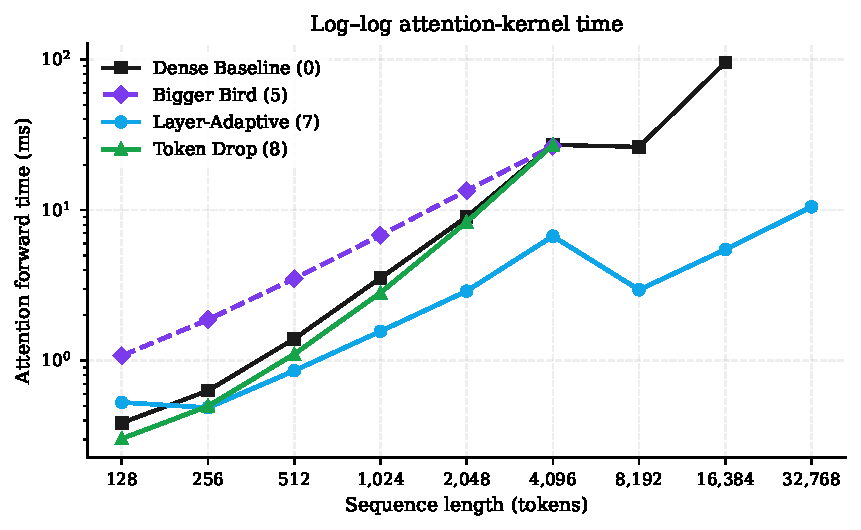
\includegraphics[width=\linewidth]{sel_loglog}
  \caption{Log--log attention-kernel time for four experiments: Dense
  Baseline (0), Bigger Bird Unified (5), Layer-Adaptive Sparsity (7), and
  Token Dropping (8). Layer-Adaptive, Token Dropping, and the dense baseline
  extend to 32{,}768 tokens; the dense baseline OOMs at that length.
  Dynamic Context (13) is absent because it was not included in the kernel
  benchmark; it appears in the efficiency figures (Figure~\ref{fig:efficiency}).
  Kernel times for all other experiments appear in Table~\ref{tab:app-kernel}.}
  \label{fig:loglog}
\end{figure}

Dense attention grows from 0.386~ms at 128 tokens to 95.4~ms at 16{,}384 and
OOMs at 32{,}768. DeepSeek Top-k, Layer-Adaptive, and GQA Sparse are
3.9--4.6$\times$ faster at 4096 tokens and about 17$\times$ faster at
16{,}384, while all complete at 32{,}768. The anomalously lower dense time at
8192 than 4096 tokens suggests a changed timing regime, so the extended sweep
supports relative ordering rather than a single fitted scaling exponent.

\begin{table}[ht]
  \centering
  \small
  \caption{Attention-forward time (ms) across nearly the full tested range,
  log-scaled sequence length. OOM denotes an out-of-memory failure.}
  \label{tab:loglog}
  \begin{tabular}{@{}rrrrr@{}}
    \toprule
    Seq.\ length & Dense (Exp 0) & DeepSeek Top-k (1) & Layer-Adaptive (7) & GQA Sparse (10) \\
    \midrule
    128    & 0.386 & 0.463 & 0.528 & 0.493 \\
    256    & 0.632 & 0.487 & 0.487 & 0.503 \\
    512    & 1.396 & 0.858 & 0.857 & 0.883 \\
    1024   & 3.537 & 1.567 & 1.567 & 1.595 \\
    2048   & 9.007 & 2.889 & 2.897 & 2.961 \\
    4096   & 27.092 & 5.834 & 6.707 & 6.925 \\
    8192   & 26.263$^\dagger$ & 2.935 & 2.953 & 3.007 \\
    16384  & 95.415 & 5.485 & 5.464 & 5.589 \\
    32768  & OOM & 10.522 & 10.504 & 10.739 \\
    \bottomrule
  \end{tabular}

  \vspace{4pt}
  \raggedright\footnotesize $^\dagger$Lower than the 4096-token value for the
  same method; see discussion of the extended-sweep discontinuity above.
\end{table}

\subsection{Linear Scale on Short and Long Sequences}

\begin{figure}[ht]
  \centering
  \begin{subfigure}[b]{0.48\linewidth}
    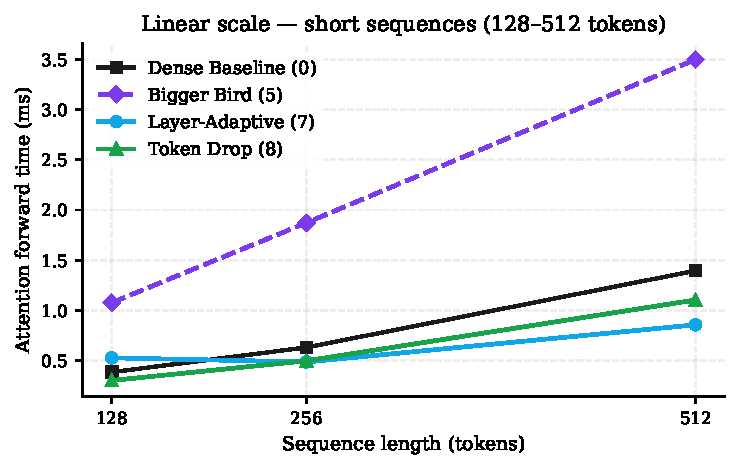
\includegraphics[width=\linewidth]{sel_linear_short}
    \caption{Short sequences (128--512 tokens).}
    \label{fig:linshort}
  \end{subfigure}
  \hfill
  \begin{subfigure}[b]{0.48\linewidth}
    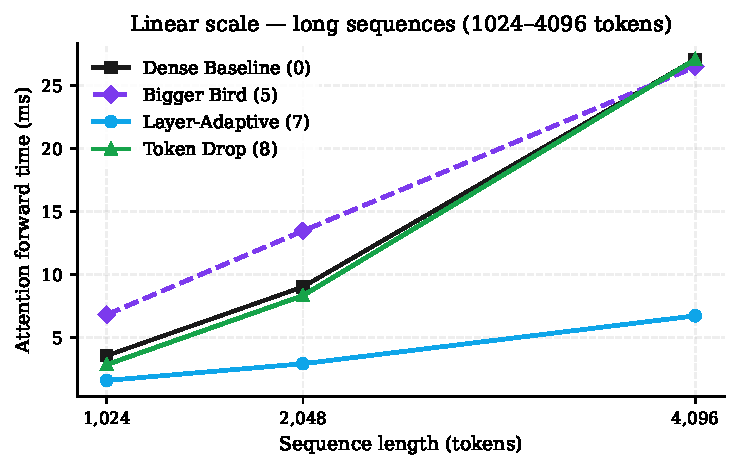
\includegraphics[width=\linewidth]{sel_linear_long}
    \caption{Long sequences (1024--4096 tokens).}
    \label{fig:linlong}
  \end{subfigure}
  \caption{Attention-kernel time on a linear scale for Dense Baseline (0),
  Bigger Bird Unified (5), Layer-Adaptive Sparsity (7), and Token Dropping (8).
  Dynamic Context (13) has no kernel benchmark and is omitted from these panels;
  it appears in Figure~\ref{fig:efficiency}. Kernel times for all other
  experiments appear in Table~\ref{tab:app-kernel}.}
  \label{fig:linear}
\end{figure}

The linear views show that routing overhead can make sparse methods slower at
128 tokens, with most crossovers occurring by 512 tokens. From 1024 to 4096,
dense time grows 7.7$\times$, compared with 3.7$\times$ for DeepSeek Top-k.

\begin{table}[ht]
  \centering
  \small
  \caption{Attention-forward time (ms), short sequences (128--512 tokens),
  linear scale.}
  \label{tab:short}
  \begin{tabular}{@{}lrrr@{}}
    \toprule
    Method & 128 & 256 & 512 \\
    \midrule
    Dense baseline (0)        & 0.386 & 0.632 & 1.396 \\
    DeepSeek Top-k (1)        & 0.463 & 0.487 & 0.858 \\
    Lightning Hybrid (2)      & 1.157 & 2.209 & 4.277 \\
    Dynamic Globals (3)       & 0.873 & 1.432 & 2.642 \\
    PBS Attn (4)              & 0.307 & 0.580 & 0.915 \\
    Bigger Bird Unified (5)   & 1.078 & 1.872 & 3.499 \\
    DeepSeek+PBS (6)          & 0.809 & 0.783 & 0.974 \\
    Layer-Adaptive (7)        & 0.528 & 0.487 & 0.857 \\
    Token Drop (8)            & 0.303 & 0.499 & 1.105 \\
    Attn Speculation (9)      & 0.745 & 1.294 & 2.433 \\
    GQA+Sparse (10)           & 0.493 & 0.503 & 0.883 \\
    \bottomrule
  \end{tabular}
\end{table}

\begin{table}[ht]
  \centering
  \small
  \caption{Attention-forward time (ms), long sequences (1024--4096 tokens),
  linear scale.}
  \label{tab:long}
  \begin{tabular}{@{}lrrr@{}}
    \toprule
    Method & 1024 & 2048 & 4096 \\
    \midrule
    Dense baseline (0)        & 3.537 & 9.007  & 27.092 \\
    DeepSeek Top-k (1)        & 1.567 & 2.889  & 5.834 \\
    Lightning Hybrid (2)      & 8.783 & 17.406 & 34.411 \\
    Dynamic Globals (3)       & 5.068 & 9.940  & 19.447 \\
    PBS Attn (4)              & 1.663 & 3.068  & 6.162 \\
    Bigger Bird Unified (5)   & 6.798 & 13.455 & 26.502 \\
    DeepSeek+PBS (6)          & 1.678 & 3.014  & 6.147 \\
    Layer-Adaptive (7)        & 1.567 & 2.897  & 6.707 \\
    Token Drop (8)            & 2.823 & 8.315  & 27.085 \\
    Attn Speculation (9)      & 4.722 & 9.451  & 18.575 \\
    GQA+Sparse (10)           & 1.595 & 2.961  & 6.925 \\
    \bottomrule
  \end{tabular}
\end{table}

Lightning Hybrid and Bigger Bird Unified remain slower than dense attention
in this range. Token Drop reaches near-dense kernel time at 4096 because its
first three layers are dense; its end-to-end advantage appears in
Section~\ref{sec:efficiency}.

\subsection{Efficiency Metrics: F1, Latency, Memory, and Training Time}
\label{sec:efficiency}

\begin{figure}[ht]
  \centering
  \begin{subfigure}[b]{0.49\linewidth}
    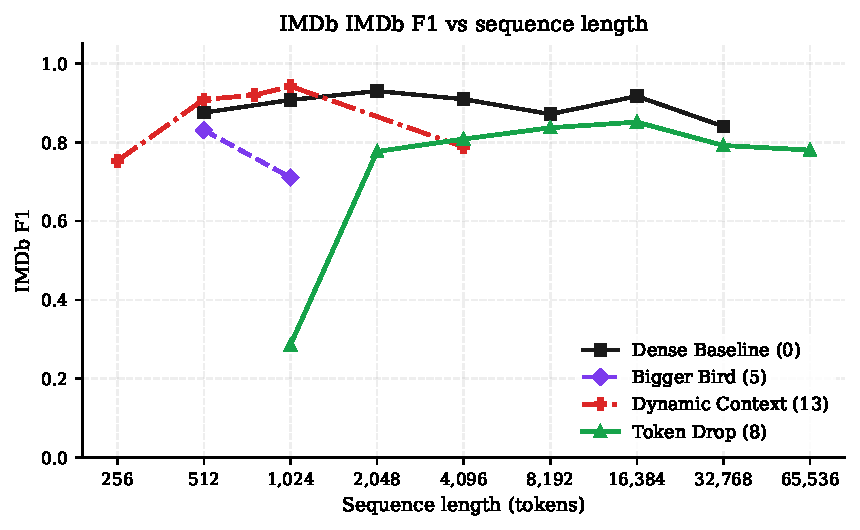
\includegraphics[width=\linewidth]{sel_f1}
    \caption{IMDb F1 vs sequence length.}
    \label{fig:f1seq}
  \end{subfigure}
  \hfill
  \begin{subfigure}[b]{0.49\linewidth}
    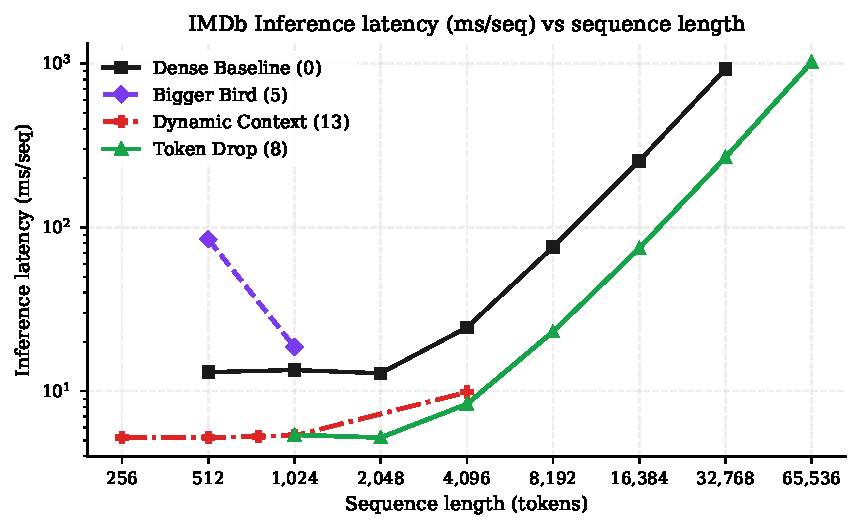
\includegraphics[width=\linewidth]{sel_latency}
    \caption{Inference latency vs sequence length.}
    \label{fig:latseq}
  \end{subfigure}

  \medskip
  \begin{subfigure}[b]{0.49\linewidth}
    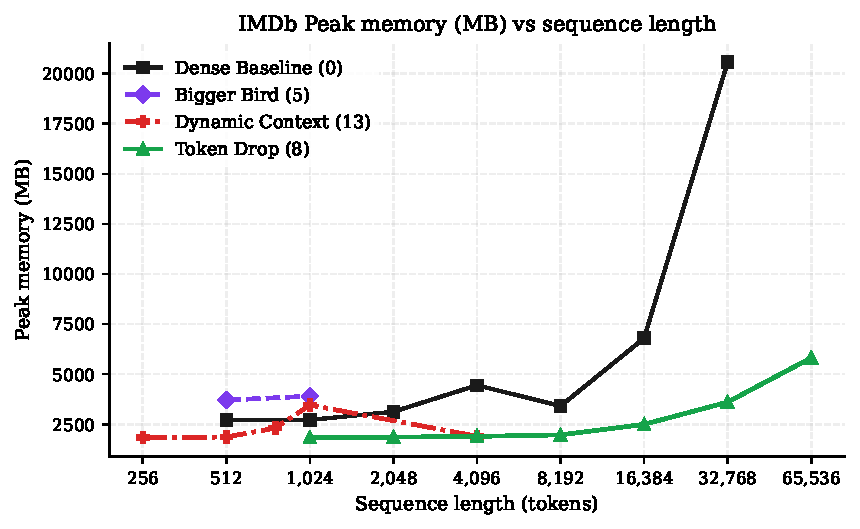
\includegraphics[width=\linewidth]{sel_memory}
    \caption{Peak device memory vs sequence length.}
    \label{fig:memseq}
  \end{subfigure}
  \hfill
  \begin{subfigure}[b]{0.49\linewidth}
    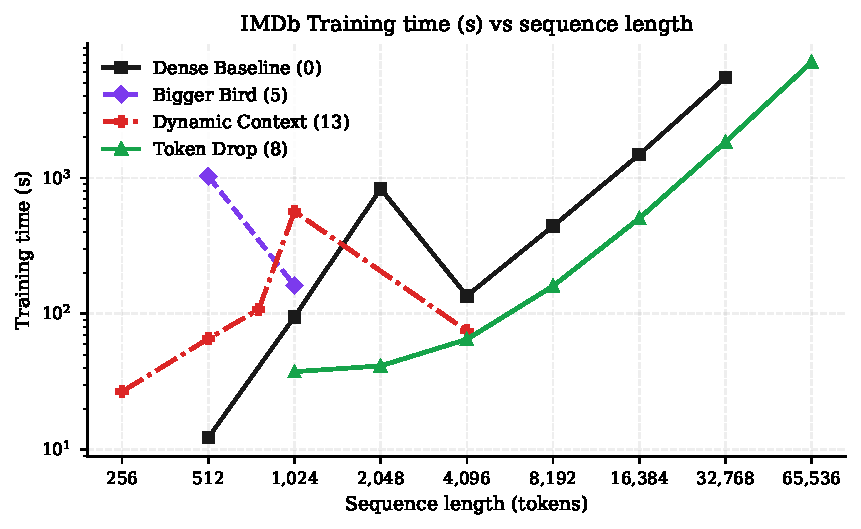
\includegraphics[width=\linewidth]{sel_traintime}
    \caption{Training time vs sequence length.}
    \label{fig:trainseq}
  \end{subfigure}

  \caption{IMDb task-level efficiency for the four highlighted experiments:
  Dense Baseline (0), Bigger Bird Unified (5), and the two top-performing
  alternatives by overall score: Dynamic Context (13) and Token Dropping (8).
  Overall score is the mean of six normalized axes --- F1, accuracy, inference
  speed, memory efficiency, training efficiency, and sparsity --- averaged
  across all recorded sequence lengths. Full results for all remaining
  experiments appear in Table~\ref{tab:app-imdb}.}
  \label{fig:efficiency}
\end{figure}

The panels compare task-level F1, latency, memory, and training time. The
detailed tables add DeepSeek Top-k because it has broad length coverage; all
other results appear in Table~\ref{tab:app-imdb}. An em-dash denotes a missing
metric, and OOM denotes an out-of-memory failure.

\begin{table}[ht]
  \centering
  \small
  \caption{Dense baseline (Experiment 0): IMDb efficiency by sequence length.}
  \label{tab:eff-baseline}
  \begin{tabular}{@{}rrrrr@{}}
    \toprule
    Seq.\ length & F1 & Train time (s) & Peak memory (MB) & Latency (ms) \\
    \midrule
    256    & 0.878 & 157.3   & ---      & ---   \\
    512    & 0.871 & 56.3    & 2707.4   & 13.68 \\
    768    & 0.931 & 216.7   & ---      & ---   \\
    1024   & 0.894 & 57.3    & 2725.4   & 13.18 \\
    2048   & 0.900 & 66.6    & 3061.0   & 13.21 \\
    4096   & 0.909 & 135.6   & 4446.4   & 24.47 \\
    8192   & 0.871 & 441.4   & 3408.8   & 75.72 \\
    16384  & 0.917 & 1484.9  & 6793.8   & 253.99 \\
    32768  & 0.840 & 5485.6  & 20{,}577.4 & 924.88 \\
    65536  & OOM   & OOM     & OOM      & OOM   \\
    \bottomrule
  \end{tabular}
\end{table}

\begin{table}[ht]
  \centering
  \small
  \caption{DeepSeek Top-k (Experiment 1): IMDb efficiency by sequence length.}
  \label{tab:eff-deepseek}
  \begin{tabular}{@{}rrrrr@{}}
    \toprule
    Seq.\ length & F1 & Train time (s) & Peak memory (MB) & Latency (ms) \\
    \midrule
    256    & 0.917 & 187.2  & ---      & ---   \\
    512    & 0.860 & 60.8   & 2701.4   & 16.07 \\
    768    & 0.926 & 609.8  & ---      & ---   \\
    1024   & 0.820 & 61.6   & 2726.6   & 15.00 \\
    2048   & 0.519 & 62.5   & 3077.6   & 15.08 \\
    4096   & 0.821 & 102.6  & 4385.7   & 20.40 \\
    8192   & 0.600 & 295.6  & 3390.2   & 53.94 \\
    16384  & 0.812 & 907.0  & 6791.6   & 168.21 \\
    32768  & 0.000 & 3170.7 & 20{,}577.1 & 581.10 \\
    65536  & OOM   & OOM    & OOM      & OOM   \\
    \bottomrule
  \end{tabular}
\end{table}

\begin{table}[ht]
  \centering
  \small
  \caption{Layer-Adaptive Sparsity (Experiment 7): IMDb efficiency by
  sequence length.}
  \label{tab:eff-layeradaptive}
  \begin{tabular}{@{}rrrrr@{}}
    \toprule
    Seq.\ length & F1 & Train time (s) & Peak memory (MB) & Latency (ms) \\
    \midrule
    512    & 0.800 & 118.1  & 2696.0   & 19.58 \\
    1024   & 0.891 & 84.5   & 2724.5   & 15.95 \\
    2048   & 0.830 & 81.3   & 2781.5   & 15.59 \\
    4096   & 0.864 & 124.6  & 2817.0   & 21.88 \\
    8192   & 0.826 & 298.1  & 3406.6   & 54.63 \\
    16384  & 0.842 & 911.5  & 6792.8   & 169.32 \\
    32768  & 0.778 & 3178.2 & 20{,}575.9 & 582.94 \\
    65536  & OOM   & OOM    & OOM      & OOM   \\
    \bottomrule
  \end{tabular}
\end{table}

\begin{table}[ht]
  \centering
  \small
  \caption{Token Dropping (Experiment 8): IMDb efficiency by sequence length.}
  \label{tab:eff-tokendrop}
  \begin{tabular}{@{}rrrrr@{}}
    \toprule
    Seq.\ length & F1 & Train time (s) & Peak memory (MB) & Latency (ms) \\
    \midrule
    1024   & 0.286 & 37.5   & 1833.6   & 5.41 \\
    2048   & 0.776 & 41.3   & 1857.3   & 5.21 \\
    4096   & 0.808 & 64.8   & 1894.2   & 8.33 \\
    8192   & 0.837 & 159.9  & 1968.2   & 23.09 \\
    16384  & 0.851 & 503.3  & 2494.4   & 74.48 \\
    32768  & 0.792 & 1837.5 & 3603.6   & 266.92 \\
    65536  & 0.780 & 7112.3 & 5815.3   & 1019.87 \\
    \bottomrule
  \end{tabular}
\end{table}

\begin{table}[ht]
  \centering
  \small
  \caption{Dynamic Context (Experiment 13): IMDb efficiency by sequence
  length.}
  \label{tab:eff-dynamiccontext}
  \begin{tabular}{@{}rrrrr@{}}
    \toprule
    Seq.\ length & F1 & Train time (s) & Peak memory (MB) & Latency (ms) \\
    \midrule
    256    & 0.000 & 26.9  & 1826.8 & 5.31 \\
    512    & 0.909 & 65.5  & 1862.3 & 5.20 \\
    768    & 0.919 & 107.4 & 2311.6 & 5.30 \\
    1024   & 0.942 & 566.4 & 3457.7 & 5.35 \\
    4096   & 0.788 & 74.9  & 1898.6 & 9.85 \\
    \bottomrule
  \end{tabular}
\end{table}

Several patterns emerge across Tables~\ref{tab:eff-baseline}--\ref{tab:eff-dynamiccontext}.
Inference latency separates the methods most clearly: Dynamic Context holds
latency in the 5.2--9.9~ms range across every tested length, roughly
2.5--26$\times$ lower than dense attention at the same length, because its
fixed post-drop token budget bounds the amount of computation regardless of
input length. Token Dropping shows the same qualitative pattern at longer
lengths, overtaking dense attention's memory profile once the sequence is long
enough that the post-drop token count is meaningfully smaller than the full
sequence (from roughly 2048 tokens onward). DeepSeek Top-k and Layer-Adaptive
Sparsity track dense attention's memory footprint closely at short-to-medium
lengths (within a few percent at 512--2048 tokens) because their savings are
concentrated in comparison count rather than in the number of activations
stored, and their latency advantage over dense attention only becomes large
at 8192 tokens and beyond (53.9--54.6~ms versus 75.7~ms).

Quality is comparatively more volatile than efficiency: three of the five
methods (DeepSeek Top-k, Layer-Adaptive, and, to a lesser extent, Token
Dropping) each have at least one sequence length where F1 drops sharply below
neighboring lengths (DeepSeek Top-k: 0.519 at 2048 tokens versus 0.820 at 1024
and 0.821 at 4096; Token Dropping: 0.286 at 1024 tokens versus 0.776 at 2048).
These dips do not follow a consistent direction with sequence length and are
most plausibly attributable to training-run variance (sample count, epoch
count, and random seed all differ across individual runs) rather than to a
property of the mechanism itself; they argue for the matched, multi-seed
re-run recommended in Section~\ref{sec:limitations}.

Table~\ref{tab:quality-1024} isolates the 1024-token comparison directly, and
Table~\ref{tab:tradeoffs} restates the same data as relative speedups and
memory reductions against the dense baseline at representative lengths.

\begin{table}[ht]
  \centering
  \small
  \caption{IMDb quality at sequence length 1024.}
  \label{tab:quality-1024}
  \begin{tabular}{@{}lrrr@{}}
    \toprule
    Method & F1 & $\Delta$F1 vs.\ dense & Accuracy \\
    \midrule
    Dense baseline & 0.894 & 0.000 & 0.900 \\
    Dynamic Context & \textbf{0.942} & +0.048 & \textbf{0.941} \\
    Layer-Adaptive & 0.891 & $-0.003$ & 0.900 \\
    Attention Speculation & 0.841 & $-0.053$ & 0.860 \\
    DeepSeek Top-k & 0.820 & $-0.074$ & 0.820 \\
    Token Drop & 0.286 & $-0.608$ & 0.600 \\
    \bottomrule
  \end{tabular}
\end{table}

\begin{table}[ht]
  \centering
  \small
  \caption{Representative quality--efficiency trade-offs relative to the dense
  baseline. Speedups above one are favorable; negative memory reduction denotes
  an increase.}
  \label{tab:tradeoffs}
  \begin{tabular}{@{}rrrcrr@{}}
    \toprule
    Length & Method & $\Delta$F1 & Inference speedup & Memory reduction & Train speedup \\
    \midrule
    1024  & Dynamic Context & +0.048 & 2.46$\times$ & $-26.9$\% & 0.10$\times$ \\
    4096  & Layer-Adaptive & $-0.045$ & 1.12$\times$ & 36.6\% & 1.09$\times$ \\
    8192  & Token Drop & $-0.034$ & 3.28$\times$ & 42.3\% & 2.76$\times$ \\
    16384 & Token Drop & $-0.066$ & 3.41$\times$ & 63.3\% & 2.95$\times$ \\
    32768 & Token Drop & $-0.048$ & 3.47$\times$ & 82.5\% & 2.99$\times$ \\
    \bottomrule
  \end{tabular}
\end{table}

Comparison count alone is not an adequate efficiency proxy. Dynamic Context at
1024 tokens reports about 1.85 billion softmax comparisons, versus 151 million
for dense attention, despite its much lower measured inference latency;
conversely, Layer-Adaptive at 4096 tokens reduces comparisons by 97.7\% but
improves end-to-end latency by only 12\%. Kernel overhead, the point at which
tokens are dropped, and the measurement boundary all need to be reported
alongside the comparison count, not in place of it.

\subsection{BigBird Family Results}
\label{sec:bigbird-family-results}

\begin{figure}[ht]
  \centering
  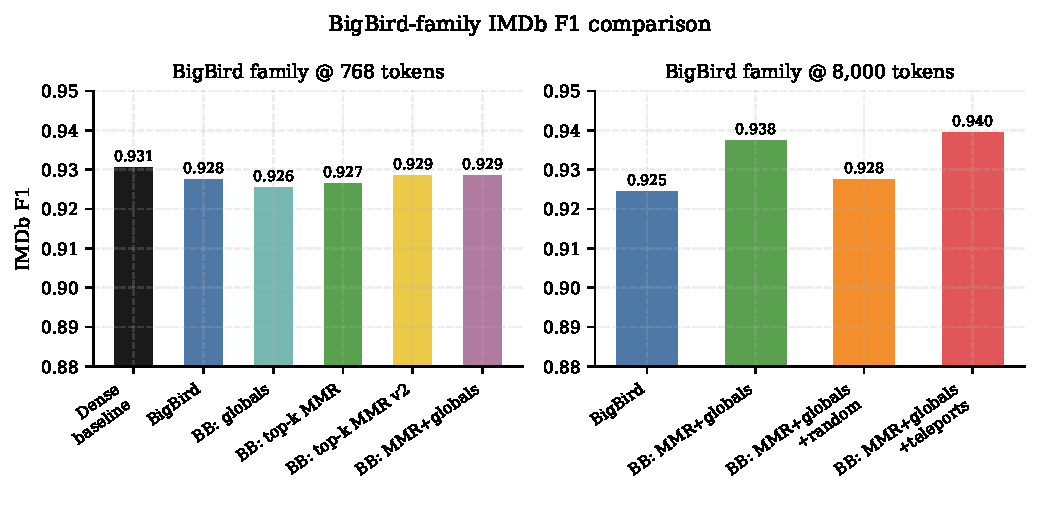
\includegraphics[width=\linewidth]{fig_bigbird_family}
  \caption{BigBird-family IMDb F1 at 768 tokens (left) and 8{,}000 tokens
  (right). All BigBird variants stay within 0.005 F1 of dense attention at
  768 tokens while training 12--14.7$\times$ slower; at 8{,}000 tokens
  the teleport-augmented variant reaches the family's best F1 (0.940) in
  4.9$\times$ less time than plain BigBird.}
  \label{fig:bigbirdfamily}
\end{figure}

Table~\ref{tab:bigbird-family} compares standard BigBird and four Bigger Bird
variants (Section~\ref{exp:bigbird-family}) against dense attention and the
unified design (Experiment~5) at 768 tokens. All BigBird-family variants land
within 0.005 F1 of dense attention, but every one of them trains
12--14.7$\times$ slower.

\begin{table}[ht]
  \centering
  \small
  \caption{BigBird-family IMDb results at sequence length 768.}
  \label{tab:bigbird-family}
  \begin{tabular}{@{}lrrr@{}}
    \toprule
    Method & F1 & Accuracy & Training time (s) \\
    \midrule
    Dense baseline & 0.931 & 0.931 & 216.7 \\
    BigBird & 0.928 & 0.931 & 2766.6 \\
    Bigger Bird: globals & 0.926 & 0.929 & 3055.8 \\
    Bigger Bird: top-k MMR & 0.927 & 0.930 & 2902.7 \\
    Bigger Bird: top-k MMR v2 & 0.929 & 0.932 & 2929.3 \\
    Bigger Bird: top-k MMR + globals & 0.929 & 0.932 & 3184.5 \\
    \bottomrule
  \end{tabular}
\end{table}

At the longer 8{,}000-token IMDb configuration, the family separates further:
BigBird reaches F1~0.925 in 21{,}504~s of training, while Bigger Bird with
top-k~MMR + globals + teleports reaches the family's best F1 (0.940) in only
4348.7~s -- a 4.9$\times$ training-time reduction over plain BigBird at
comparable or better quality (Table~\ref{tab:bigbird-8000}).

\begin{table}[ht]
  \centering
  \small
  \caption{BigBird-family IMDb results at sequence length 8000.}
  \label{tab:bigbird-8000}
  \begin{tabular}{@{}lrrr@{}}
    \toprule
    Method & F1 & Accuracy & Training time (s) \\
    \midrule
    BigBird & 0.925 & 0.928 & 21{,}504.5 \\
    Bigger Bird: top-k MMR + globals & 0.938 & 0.940 & 7484.3 \\
    Bigger Bird: top-k MMR + globals + random & 0.928 & 0.930 & 5832.9 \\
    Bigger Bird: top-k MMR + globals + teleports & \textbf{0.940} & \textbf{0.941} & \textbf{4348.7} \\
    \bottomrule
  \end{tabular}
\end{table}

\section{Discussion}

Kernel sparsity does not guarantee task-level efficiency. Layer-Adaptive best
combines speed and stable IMDb quality; Token Dropping gives the strongest
long-context latency and memory results and is the only method validated at
65{,}536 tokens. Dynamic Context has the best short-context quality but high
training cost. Teleport-augmented Bigger Bird improves both F1 and training
time over plain BigBird at 8000 tokens (Table~\ref{tab:bigbird-8000}).

\section{Limitations}
\label{sec:limitations}

Training budgets, sample counts, sequence coverage, and recorded metrics are
uneven, and results are single runs without cross-seed uncertainty. The
long-context kernel sweep may use a different timing regime, while LRA and
RULER results remain exploratory. Bigger Bird and Experiment~14 were also
evaluated under different settings and metrics, so their charts should be
regenerated before direct comparison.

Experiments 11 and 12 are unfinished. In addition, ``Bigger Bird'' refers to
distinct BART and BigBird-RoBERTa implementations plus a related BART ablation;
comparisons should use experiment numbers and backbones. Timing and memory
results are specific to the recorded CUDA hardware.


\clearpage
\appendix
\section*{Appendix: Developmental Encoder Full Tables}
\addcontentsline{toc}{section}{Appendix: Developmental Encoder Full Tables}

This appendix reports the full IMDb / kernel tables from the early architecture
search (Section~\ref{sec:developmental}). These smaller-scale runs support
design rationale and scaling trends; they are not the primary R1 long-context
evidence. Experiments highlighted in the developmental section are: Dense
Baseline (0), Bigger Bird Unified (5), Dynamic Context (13), and Token
Dropping (8).

\subsection*{A.1\quad Attention-Kernel Forward Time (ms)}
OOM denotes an out-of-memory failure; `---' denotes not benchmarked at that length.

\begin{table}[ht]
  \centering
  \small
  \caption{Attention-kernel forward time (ms) for omitted experiments, 128--4096 tokens.}
  \label{tab:app-kernel}
  \begin{tabular}{@{}lrrrrrr@{}}
    \toprule
    Experiment & 128 & 256 & 512 & 1,024 & 2,048 & 4,096 \\
    \midrule
    GQA+Sparse & 0.493 & 0.503 & 0.883 & 1.595 & 2.961 & 6.925 \\
    DeepSeek Top-k & 0.463 & 0.487 & 0.858 & 1.567 & 2.889 & 5.834 \\
    Lightning Hybrid & 1.157 & 2.209 & 4.277 & 8.783 & 17.406 & 34.411 \\
    Dynamic Global Tokens & 0.873 & 1.432 & 2.642 & 5.068 & 9.940 & 19.447 \\
    PBS Attention & 0.307 & 0.580 & 0.915 & 1.663 & 3.068 & 6.162 \\
    DeepSeek+PBS Hybrid & 0.809 & 0.783 & 0.974 & 1.678 & 3.014 & 6.147 \\
    Attention Speculation & 0.745 & 1.294 & 2.433 & 4.722 & 9.451 & 18.575 \\
    \bottomrule
  \end{tabular}
\end{table}

\FloatBarrier

\subsection*{A.2\quad IMDb Task-Level Results (All Sequence Lengths)}
F1 = 0.000 with accuracy $\approx$ 0.53 indicates majority-class collapse.
OOM rows are included where recorded. `---' denotes metric not recorded.

\begingroup
\small
\setlength{\tabcolsep}{3pt}
\renewcommand{\addlinespace}[1][]{}
\newenvironment{appresultstable}{%
  \begin{center}
  \begin{tabular}{@{}>{\raggedright\arraybackslash}p{0.35\textwidth}lrrrrr@{}}
  \toprule
  Experiment & Seq & F1 & Acc & Train (s) & Mem. (MB) & Lat. (ms) \\
  \midrule
}{%
  \end{tabular}
  \end{center}
}
\captionsetup{hypcap=false}
\captionof{table}{IMDb task-level results for all experiments not in the main figures.}
\label{tab:app-imdb}
\begin{appresultstable}
  DeepSeek Top-k & 256 & 0.677 & 0.580 & 223.7 & --- & --- \\
   & 512 & 0.860 & 0.860 & 60.8 & 2701 & 16.07 \\
   & 1,024 & 0.846 & 0.840 & 100.5 & 2718 & 15.78 \\
   & 2,048 & 0.873 & 0.873 & 678.1 & 3124 & 15.30 \\
   & 4,096 & 0.837 & 0.840 & 131.5 & 2815 & 20.69 \\
   & 8,192 & 0.600 & 0.680 & 295.6 & 3390 & 53.94 \\
   & 16,384 & 0.812 & 0.820 & 907.0 & 6792 & 168.21 \\
   & 32,768 & 0.000 & 0.530 & 3170.7 & 20577 & 581.10 \\
   & 65,536 & \multicolumn{5}{l}{OOM} \\
  \addlinespace[4pt]
  Lightning Hybrid & 256 & 0.000 & 0.530 & 49.7 & 2806 & 47.37 \\
   & 512 & 0.775 & 0.770 & 10731.5 & 6034 & 73.68 \\
   & 1,024 & 0.750 & 0.600 & 2.3 & 2793 & 20.38 \\
   & 2,048 & 0.829 & 0.832 & 2603.4 & 7423 & 28.68 \\
   & 4,096 & 0.621 & 0.670 & 274.4 & 13956 & 52.25 \\
  \addlinespace[4pt]
\end{appresultstable}
\clearpage
\begin{appresultstable}
  Dynamic Global Tokens & 256 & 0.541 & 0.660 & 278.2 & --- & --- \\
   & 1,024 & 0.295 & 0.570 & 123.7 & 2716 & 18.54 \\
   & 2,048 & 0.840 & 0.842 & 2144.3 & 4999 & 21.33 \\
   & 4,096 & 0.000 & 0.530 & 281.8 & 3512 & 36.92 \\
  \addlinespace[4pt]
  PBS Attention & 256 & 0.550 & 0.640 & 317.2 & --- & --- \\
   & 512 & 0.000 & 0.560 & 13.1 & 2705 & 15.52 \\
   & 1,024 & 0.000 & 0.530 & 104.7 & 2716 & 15.37 \\
   & 2,048 & 0.656 & 0.488 & 698.5 & 3132 & 15.81 \\
   & 4,096 & 0.000 & 0.530 & 132.7 & 2815 & 21.12 \\
  \addlinespace[4pt]
  DeepSeek+PBS Hybrid & 512 & 0.000 & 0.530 & 128.0 & 2696 & 20.50 \\
   & 1,024 & \multicolumn{5}{l}{OOM} \\
   & 2,048 & \multicolumn{5}{l}{OOM} \\
   & 4,096 & \multicolumn{5}{l}{OOM} \\
  \addlinespace[4pt]
  Layer-Adaptive Sparsity & 512 & 0.848 & 0.850 & 99.2 & 2696 & 14.70 \\
   & 1,024 & 0.891 & 0.900 & 84.5 & 2725 & 15.95 \\
   & 2,048 & 0.901 & 0.901 & 687.5 & 3120 & 15.02 \\
   & 4,096 & 0.864 & 0.880 & 124.6 & 2817 & 21.88 \\
   & 8,192 & 0.826 & 0.840 & 298.1 & 3407 & 54.63 \\
   & 16,384 & 0.842 & 0.850 & 911.5 & 6793 & 169.32 \\
   & 32,768 & 0.778 & 0.800 & 3178.2 & 20576 & 582.94 \\
   & 65,536 & \multicolumn{5}{l}{OOM} \\
  \addlinespace[4pt]
  Attention Speculation & 1,024 & 0.841 & 0.860 & 132.5 & 4113 & 16.61 \\
   & 2,048 & 0.860 & 0.860 & 253.4 & 9395 & 21.00 \\
   & 4,096 & \multicolumn{5}{l}{OOM} \\
  \addlinespace[4pt]
  GQA+Sparse & 512 & 0.000 & 0.530 & 119.6 & 2696 & 19.63 \\
   & 1,024 & 0.763 & 0.770 & 107.2 & 2714 & 15.50 \\
   & 2,048 & 0.796 & 0.800 & 121.5 & 2779 & 21.95 \\
   & 4,096 & 0.750 & 0.800 & 123.2 & 2817 & 22.30 \\
  \addlinespace[4pt]
  Native Sparse Attn (NSA) & \multicolumn{6}{l}{No task-level run recorded} \\
  S2-HHST & \multicolumn{6}{l}{No task-level run recorded} \\
  Token Drop + DeepSeek & 4,096 & 0.641 & 0.485 & 67.9 & 17100 & 17.61 \\
   & 8,192 & 0.041 & 0.530 & 246.6 & 33011 & 62.81 \\
   & 16,384 & \multicolumn{5}{l}{OOM} \\
   & 32,768 & \multicolumn{5}{l}{OOM} \\
   & 65,536 & \multicolumn{5}{l}{OOM} \\
  \addlinespace[4pt]
  Bigger Bird (BigBird-RoBERTa) & \multicolumn{6}{l}{No task-level run recorded} \\
\end{appresultstable}
\clearpage
\begin{appresultstable}
  lra_text_exp_7_layer_adaptive & 512 & 0.649 & 0.480 & 60.7 & 950 & 15.02 \\
   & 1,024 & 0.649 & 0.480 & 123.1 & 1527 & 24.06 \\
   & 2,048 & 0.649 & 0.480 & 263.5 & 2724 & 51.59 \\
   & 4,096 & 0.649 & 0.480 & 26.2 & 3868 & 8.54 \\
   & 8,192 & 0.000 & 0.438 & 37.6 & 2902 & 259.83 \\
   & 16,384 & 0.000 & 0.520 & 199.5 & 2586 & 20.67 \\
   & 32,768 & 0.000 & 0.520 & 542.9 & 6836 & 45.89 \\
  \addlinespace[4pt]
  lra_text_exp_11_nsa & 1,024 & 0.000 & 0.438 & 797.4 & 8941 & 79.09 \\
  \addlinespace[4pt]
  lra_listops_exp_11_nsa & 512 & 0.060 & 0.135 & 9541.5 & 15508 & 40.18 \\
  \addlinespace[4pt]
  ruler_niah_exp_2_lightning_hybrid & 4,096 & 0.016 & 0.085 & 900.0 & 30138 & 43.10 \\
   & 8,192 & 0.021 & 0.120 & 1815.4 & 30202 & 93.09 \\
   & 16,384 & 0.017 & 0.090 & 4140.7 & 7365 & 196.94 \\
  \addlinespace[4pt]
  lra_listops_exp_2_lightning_hybrid & 512 & 0.024 & 0.135 & 1249.1 & 7475 & 24.37 \\
   & 1,024 & 0.023 & 0.130 & 4093.7 & 14799 & 48.17 \\
  \addlinespace[4pt]
  ruler_niah_exp_1_deepseek_topk & 4,096 & 0.016 & 0.085 & 52.9 & 3530 & 8.32 \\
   & 8,192 & 0.021 & 0.120 & 113.2 & 3601 & 9.78 \\
   & 16,384 & 0.017 & 0.090 & 344.9 & 1562 & 20.02 \\
   & 32,768 & 0.019 & 0.105 & 770.5 & 2740 & 44.49 \\
  \addlinespace[4pt]
  lra_text_exp_3_dynamic_globals & 1,024 & 0.000 & 0.438 & 10.4 & 2170 & 35.91 \\
   & 2,048 & 0.000 & 0.438 & 16.9 & 4032 & 76.44 \\
   & 4,096 & 0.000 & 0.438 & 363.6 & 7739 & 162.47 \\
   & 8,192 & 0.000 & 0.438 & 922.9 & 15164 & 363.20 \\
  \addlinespace[4pt]
  lra_text_exp_14_token_drop_deepseek & 4,096 & 0.641 & 0.485 & 67.9 & 17100 & 17.61 \\
   & 8,192 & 0.041 & 0.530 & 246.6 & 33011 & 62.81 \\
  \addlinespace[4pt]
  ruler_niah_exp_7_layer_adaptive & 4,096 & 0.016 & 0.085 & 54.6 & 3676 & 9.06 \\
   & 8,192 & 0.021 & 0.120 & 118.7 & 3746 & 10.35 \\
   & 16,384 & 0.017 & 0.090 & 348.7 & 1562 & 20.60 \\
  \addlinespace[4pt]
  biggerbird_topk_mmr & 768 & 0.927 & 0.930 & 2902.7 & --- & --- \\
  \addlinespace[4pt]
  lra_text_exp_12_s2_hhst & 1,024 & 0.000 & 0.438 & 318.9 & 6532 & 50.45 \\
  \addlinespace[4pt]
  lra_listops_exp_3_dynamic_globals & 512 & 0.034 & 0.140 & 166.3 & 4076 & 20.28 \\
   & 1,024 & 0.023 & 0.130 & 3705.6 & 7760 & 35.03 \\
  \addlinespace[4pt]
\end{appresultstable}
\clearpage
\begin{appresultstable}
  lra_listops_exp_5_bigger_bird & 512 & 0.042 & 0.135 & 1090.2 & 5548 & 25.30 \\
   & 1,024 & 0.030 & 0.135 & 8795.5 & 14803 & 45.27 \\
  \addlinespace[4pt]
  lra_listops_exp_10_gqa_sparse & 512 & 0.033 & 0.140 & 59.9 & 950 & 18.25 \\
  \addlinespace[4pt]
  biggerbird_topkmmr+globals_ver1 & 768 & 0.929 & 0.932 & 3184.5 & --- & --- \\
  \addlinespace[4pt]
  lra_listops_exp_12_s2_hhst & 512 & 0.068 & 0.150 & 5728.8 & 9454 & 24.35 \\
  \addlinespace[4pt]
  ruler_niah_exp_6_deepseek_pbs & 4,096 & 0.016 & 0.085 & 53.6 & 3530 & 10.43 \\
   & 8,192 & 0.021 & 0.120 & 115.6 & 3601 & 11.70 \\
   & 16,384 & 0.017 & 0.090 & 357.2 & 1562 & 20.58 \\
  \addlinespace[4pt]
  lra_listops_exp_7_layer_adaptive & 256 & 0.023 & 0.133 & 11.2 & 841 & 12.20 \\
   & 512 & 0.052 & 0.140 & 60.6 & 949 & 17.00 \\
   & 1,024 & 0.023 & 0.130 & 122.7 & 1526 & 24.34 \\
   & 2,048 & 0.019 & 0.105 & 263.3 & 2722 & 51.68 \\
  \addlinespace[4pt]
  lra_text_exp_0_baseline & 256 & 0.646 & 0.477 & 44.5 & 684 & 28.36 \\
   & 512 & 0.649 & 0.480 & 71.0 & 946 & 14.24 \\
   & 1,024 & 0.649 & 0.480 & 170.2 & 1561 & 26.54 \\
   & 2,048 & 0.667 & 0.500 & 20.7 & 2955 & 67.15 \\
   & 4,096 & 0.000 & 0.438 & 33.1 & 1840 & 188.13 \\
   & 8,192 & 0.000 & 0.438 & 110.5 & 4293 & 582.79 \\
  \addlinespace[4pt]
  ruler_niah_exp_13_dynamic_context & 4,096 & 1.000 & 1.000 & 83.3 & 2646 & 7.70 \\
   & 8,192 & 0.021 & 0.120 & 185.9 & 2115 & 13.93 \\
   & 16,384 & 0.017 & 0.090 & 457.9 & 906 & 23.84 \\
   & 32,768 & 0.019 & 0.105 & 829.0 & 1283 & 43.44 \\
   & 65,536 & 0.021 & 0.120 & 1612.0 & 2005 & 82.77 \\
  \addlinespace[4pt]
  lra_text_exp_5_bigger_bird & 1,024 & 0.000 & 0.438 & 71.6 & 3930 & 45.84 \\
   & 2,048 & 0.000 & 0.438 & 701.2 & 11646 & 128.71 \\
  \addlinespace[4pt]
  lra_text_exp_2_lightning_hybrid & 1,024 & 0.000 & 0.438 & 12.2 & 3934 & 50.24 \\
   & 2,048 & 0.000 & 0.438 & 148.2 & 7546 & 122.45 \\
   & 4,096 & 0.649 & 0.480 & 356.4 & 30144 & 44.26 \\
   & 8,192 & 0.000 & 0.520 & 733.2 & 30210 & 93.02 \\
   & 32,768 & 0.000 & 0.520 & 3523.6 & 15374 & 401.49 \\
  \addlinespace[4pt]
  biggerbird_topkMMR_globals_teleports_8000 & 8,000 & 0.940 & 0.941 & 4348.7 & --- & --- \\
  \addlinespace[4pt]
  ruler_niah_exp_0_baseline & 512 & 0.027 & 0.156 & 525.0 & 0 & 247.83 \\
  \addlinespace[4pt]
  biggerbird_topk_mmr_ver2_(kaggle) & 768 & 0.929 & 0.932 & 2929.3 & --- & --- \\
  \addlinespace[4pt]
\end{appresultstable}
\clearpage
\begin{appresultstable}
  lra_text_exp_10_gqa_sparse & 1,024 & 0.000 & 0.438 & 4.2 & 584 & 23.22 \\
   & 2,048 & 0.000 & 0.438 & 7.3 & 884 & 49.24 \\
   & 4,096 & 0.000 & 0.438 & 15.1 & 1505 & 109.26 \\
   & 8,192 & 0.000 & 0.438 & 37.2 & 2853 & 257.82 \\
  \addlinespace[4pt]
  lra_text_exp_4_pbs_attn & 1,024 & 0.000 & 0.438 & 4.5 & 598 & 26.95 \\
   & 2,048 & 0.000 & 0.438 & 7.5 & 910 & 52.18 \\
   & 4,096 & 0.000 & 0.438 & 15.3 & 1554 & 111.76 \\
   & 8,192 & 0.000 & 0.438 & 37.8 & 2951 & 262.26 \\
  \addlinespace[4pt]
  lra_text_exp_9_attn_specul & 1,024 & 0.000 & 0.438 & 86.6 & 4294 & 35.00 \\
   & 2,048 & 0.000 & 0.438 & 641.3 & 12533 & 73.89 \\
  \addlinespace[4pt]
  lra_text_exp_8_token_drop & 512 & 0.649 & 0.480 & 47.5 & 890 & 10.50 \\
   & 1,024 & 0.649 & 0.480 & 109.8 & 1874 & 22.43 \\
   & 2,048 & 0.639 & 0.470 & 767.6 & 5221 & 62.11 \\
   & 4,096 & 0.649 & 0.480 & 98.2 & 20576 & 25.80 \\
   & 8,192 & 0.000 & 0.438 & 587.9 & 16040 & 2258.95 \\
  \addlinespace[4pt]
  ruler_niah_exp_14_token_drop_deepseek & 4,096 & 0.118 & 0.200 & 163.4 & 17100 & 17.62 \\
   & 8,192 & 0.021 & 0.120 & 588.4 & 33011 & 62.82 \\
  \addlinespace[4pt]
  lra_listops_exp_1_deepseek_topk & 256 & 0.016 & 0.086 & 11.3 & 841 & 11.91 \\
   & 512 & 0.024 & 0.135 & 60.6 & 950 & 21.29 \\
   & 1,024 & 0.033 & 0.105 & 121.3 & 1516 & 22.90 \\
   & 2,048 & 0.019 & 0.105 & 260.3 & 2669 & 51.06 \\
  \addlinespace[4pt]
  lra_text_exp_1_deepseek_topk & 256 & 0.000 & 0.523 & 11.1 & 842 & 14.95 \\
   & 512 & 0.649 & 0.480 & 61.1 & 951 & 15.14 \\
   & 1,024 & 0.649 & 0.480 & 122.8 & 1518 & 23.34 \\
   & 2,048 & 0.649 & 0.480 & 260.8 & 2671 & 51.07 \\
   & 4,096 & 0.649 & 0.480 & 25.5 & 3722 & 8.49 \\
   & 8,192 & 0.000 & 0.520 & 58.7 & 3985 & 9.75 \\
   & 16,384 & 0.000 & 0.520 & 194.5 & 2586 & 20.00 \\
   & 32,768 & 0.000 & 0.520 & 535.0 & 6836 & 44.47 \\
  \addlinespace[4pt]
  ruler_mq_niah_exp_13_dynamic_context & 4,096 & 1.000 & 1.000 & 84.6 & 2646 & 7.65 \\
   & 8,192 & 0.026 & 0.150 & 169.6 & 3769 & 13.93 \\
   & 16,384 & 0.017 & 0.090 & 300.5 & 6126 & 23.83 \\
   & 32,768 & 0.028 & 0.085 & 560.8 & 10747 & 43.51 \\
   & 65,536 & 0.017 & 0.095 & 1081.7 & 19987 & 82.70 \\
  \addlinespace[4pt]
  lra_listops_exp_4_pbs_attn & 512 & 0.025 & 0.090 & 61.3 & 980 & 16.99 \\
   & 1,024 & 0.023 & 0.130 & 121.6 & 1571 & 23.22 \\
  \addlinespace[4pt]
\end{appresultstable}
\clearpage
\begin{appresultstable}
  biggerbird_globals_ver1_(kaggle) & 768 & 0.926 & 0.929 & 3055.8 & --- & --- \\
  \addlinespace[4pt]
  ruler_niah_exp_8_token_drop & 4,096 & 0.016 & 0.085 & 236.0 & 20576 & 25.84 \\
  \addlinespace[4pt]
  biggerbird_topkMMR_globals_8000 & 8,000 & 0.938 & 0.940 & 7484.3 & --- & --- \\
  \addlinespace[4pt]
  lra_text_exp_13_dynamic_context & 4,096 & 0.641 & 0.480 & 33.7 & 2646 & 7.64 \\
   & 8,192 & 0.040 & 0.525 & 73.7 & 2115 & 13.91 \\
   & 16,384 & 0.078 & 0.530 & 180.0 & 906 & 23.86 \\
   & 32,768 & 0.020 & 0.520 & 325.6 & 1283 & 43.49 \\
   & 65,536 & 0.161 & 0.530 & 631.7 & 2005 & 82.76 \\
  \addlinespace[4pt]
  lra_listops_exp_6_deepseek_pbs & 512 & 0.025 & 0.090 & 60.5 & 950 & 17.24 \\
   & 1,024 & 0.052 & 0.165 & 119.6 & 1516 & 24.19 \\
  \addlinespace[4pt]
  lra_listops_exp_9_attn_specul & 512 & 0.016 & 0.085 & 1949.2 & 6188 & 19.69 \\
  \addlinespace[4pt]
  ruler_mq_niah_exp_8_token_drop & 4,096 & 0.021 & 0.120 & 236.9 & 20576 & 25.86 \\
  \addlinespace[4pt]
  lra_listops_exp_0_baseline & 256 & 0.023 & 0.133 & 44.5 & 683 & 28.91 \\
   & 512 & 0.018 & 0.095 & 70.1 & 944 & 14.08 \\
   & 1,024 & 0.025 & 0.140 & 168.6 & 1559 & 26.17 \\
   & 2,048 & 0.019 & 0.105 & 465.9 & 2953 & 68.99 \\
  \addlinespace[4pt]
  biggerbird_topkMMR_globals_randoms_8000 & 8,000 & 0.928 & 0.930 & 5832.9 & --- & --- \\
  \addlinespace[4pt]
  lra_listops_exp_8_token_drop & 512 & 0.044 & 0.115 & 46.5 & 888 & 10.30 \\
   & 1,024 & 0.046 & 0.140 & 109.5 & 1872 & 22.40 \\
   & 2,048 & 0.037 & 0.115 & 724.6 & 5219 & 62.24 \\
  \addlinespace[4pt]
  bigbird & 768 & 0.928 & 0.931 & 2766.6 & --- & --- \\
  \addlinespace[4pt]
  ruler_mq_niah_exp_14_token_drop_deepseek & 4,096 & 0.319 & 0.445 & 163.1 & 17100 & 17.63 \\
  \addlinespace[4pt]
  lra_text_exp_6_deepseek_pbs & 1,024 & 0.000 & 0.438 & 4.9 & 584 & 24.75 \\
   & 2,048 & 0.000 & 0.438 & 7.6 & 884 & 51.94 \\
   & 4,096 & 0.649 & 0.480 & 25.8 & 3722 & 10.20 \\
   & 8,192 & 0.000 & 0.520 & 59.9 & 3985 & 10.91 \\
   & 16,384 & 0.000 & 0.520 & 201.7 & 2586 & 20.33 \\
   & 32,768 & 0.000 & 0.520 & 537.2 & 6836 & 45.15 \\
  \addlinespace[4pt]
  bigbird_8000 & 8,000 & 0.925 & 0.928 & 21504.5 & --- & --- \\
  \addlinespace[4pt]
\end{appresultstable}
\endgroup


\end{document}